%!TEX root = ../thesis.tex
\chapter{Methods}
\label{ch:methods}

\todo{Use model project overview graphic (?)}
\section{Approach}	
In this chapter, we detail the methodology used to address the objectives we defined in the introduction.
We initially provide a quick overview of the complete Simulink model, followed by more elaborate explanations of the individual components.
Recognizing that controller and RL setup both depend on a solid, well-functioning model, we begin with a description of the hexapod representation we created in Simulink.
Subsequently, we shift focus towards the static gait motion controller, providing insights into both the trajectory generation and custom Inverse Kinematics solver.
The chapter concludes with an exploration of the RL setup we developed to train an agent on leg coordination/ gait generation.

\section{Simulink Model}

\begin{figure}[h]
	\centerline{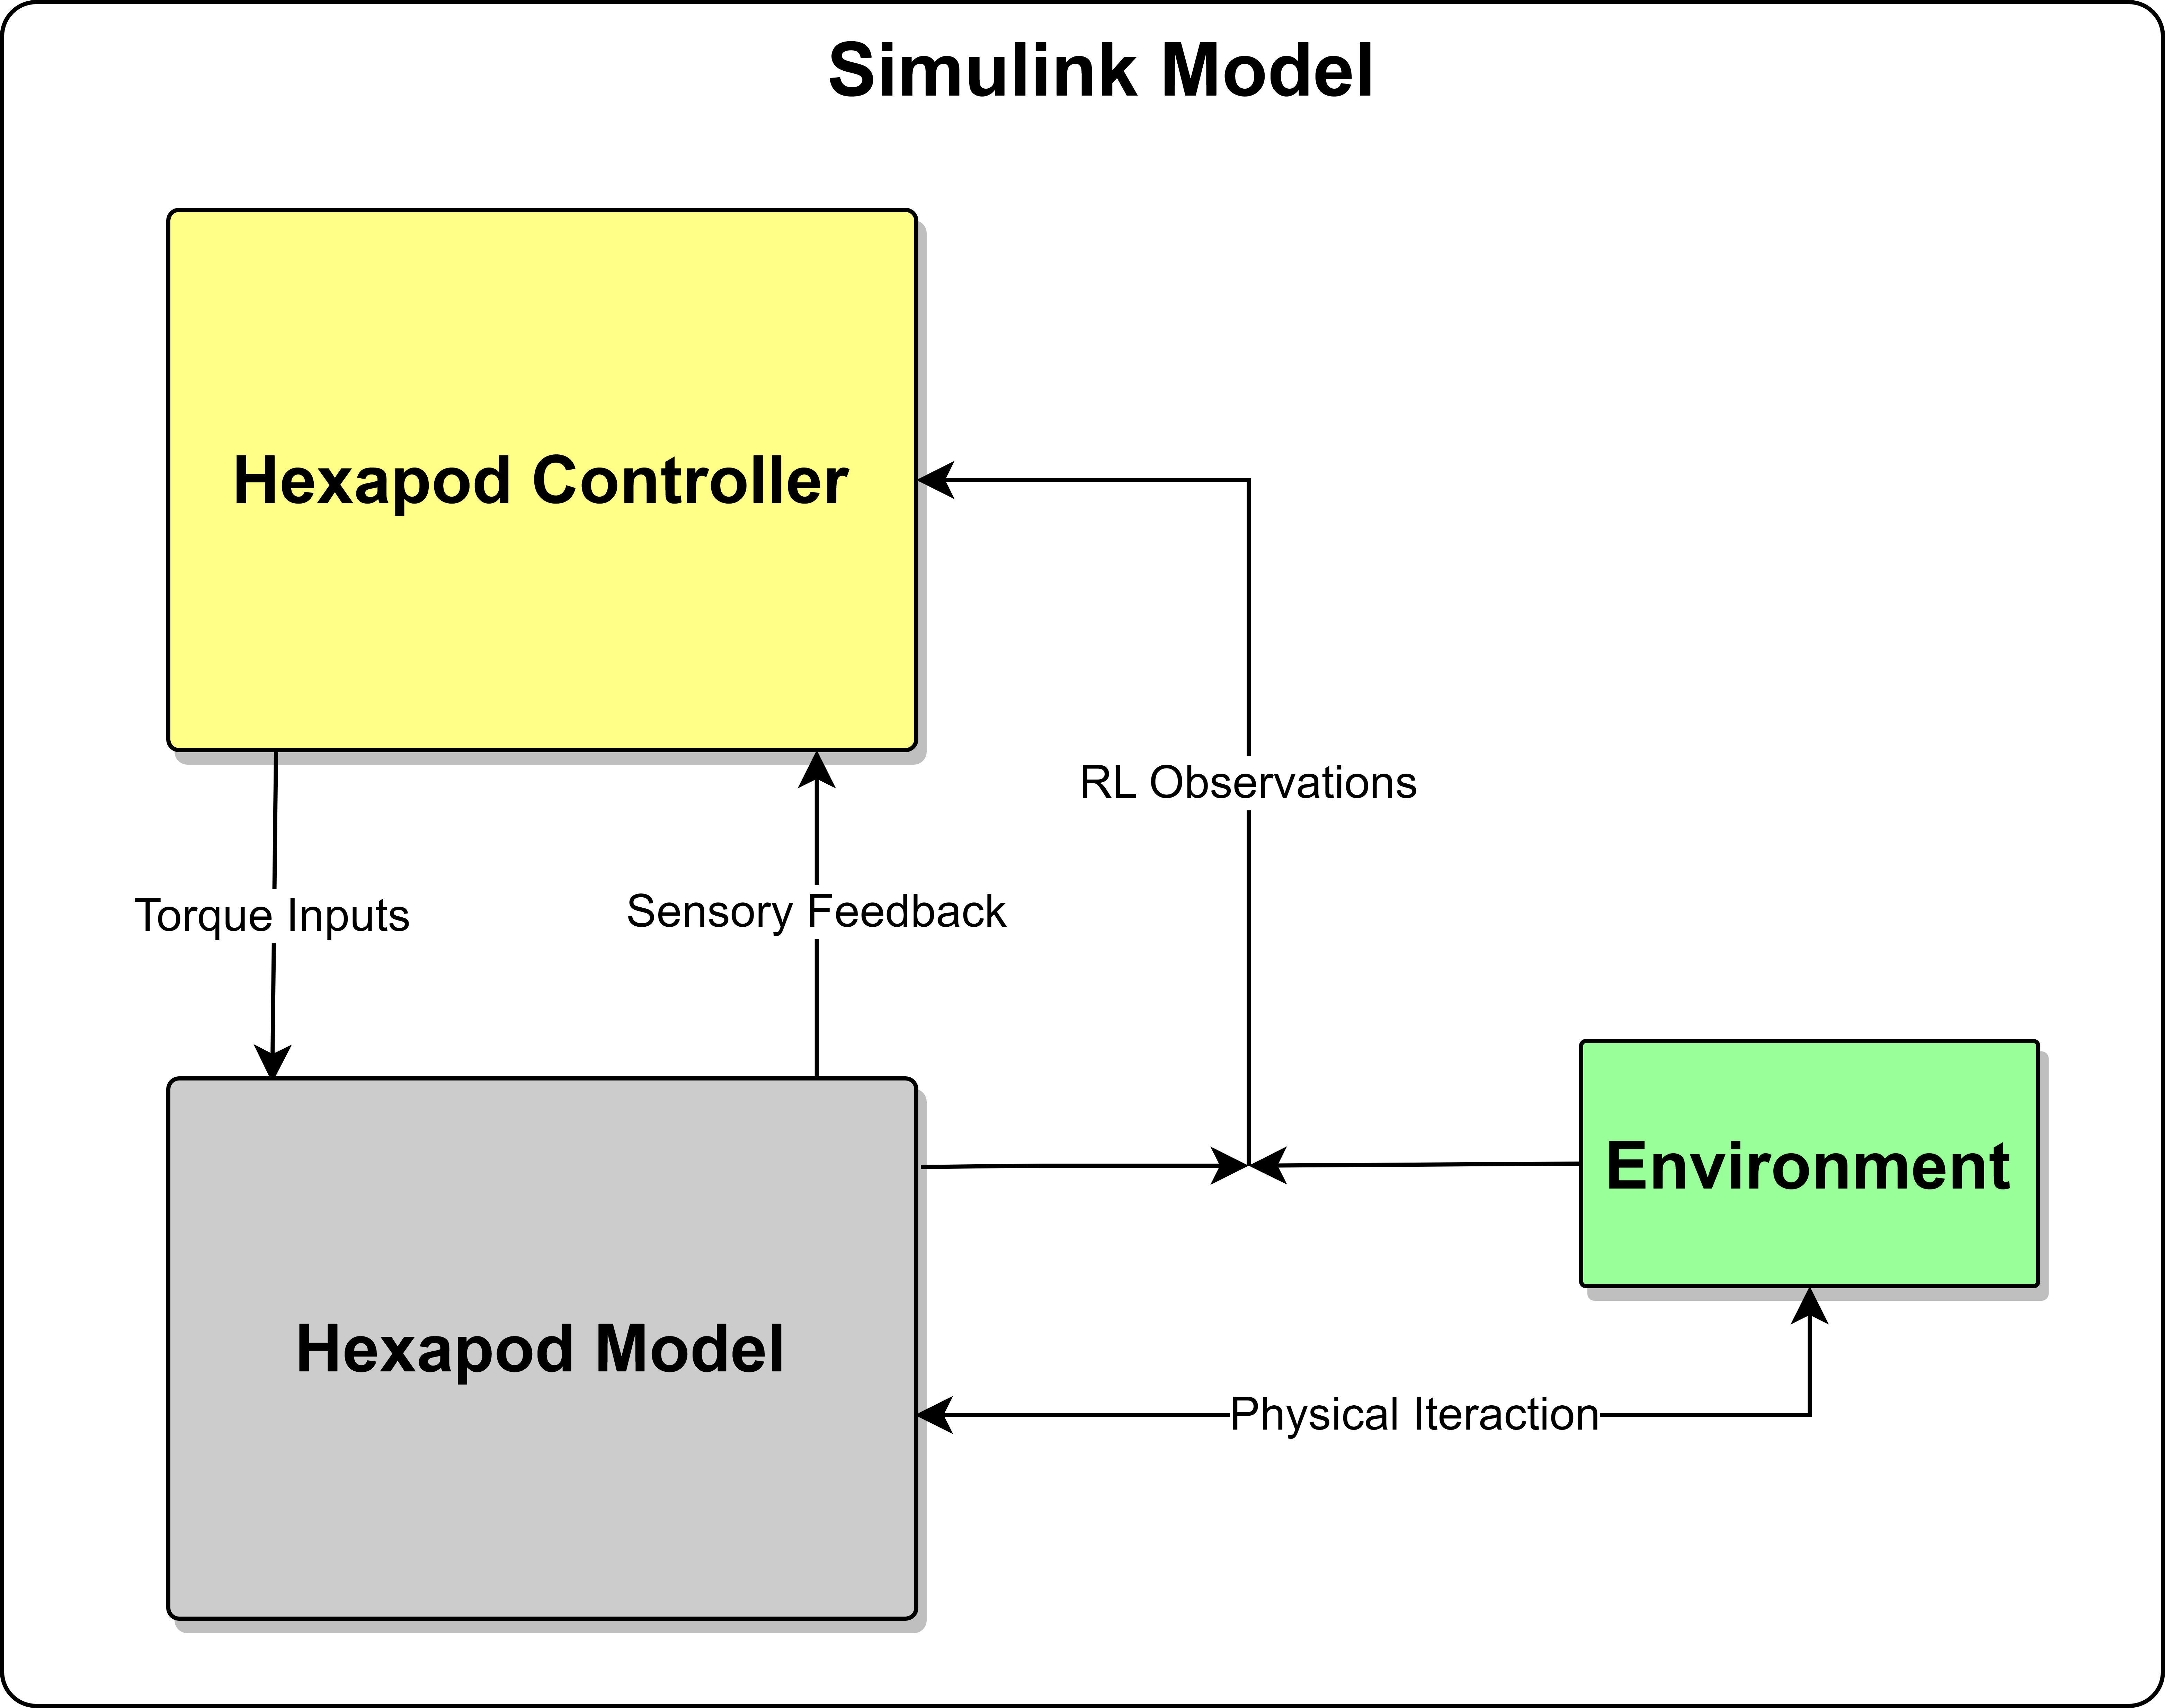
\includegraphics[scale=0.045]{HexapodModel_Overview}}
	\caption[]{Simulink model vverview}
	\label{figure: Simulink Model Overview}
\end{figure}

Taking a top-down perspective on the Simulink model as depicted in Fig. \ref{figure: Simulink Model Overview}, it is distinctly divided into 3 separate components: The hexapod, the locomotion controller and the environment.
The hexapod represents a virtual model of a real hexapod robot and together with the controller constitutes a feedback loop.
Providing sensory information about its state to the controller, the hexapod receives instructions on the torque values to be applied in return.
The environment represents a virtual testing ground in which the hexapod is situated.
Between the two components physical interactions are simulated.
Additionally, if a RL agent is supposed to be trained, both the hexapod and the environment provide so called RL observations to the controller, which RL agent setup is a part of.


\subsection{The Hexapod}
The hexapod model we develop in this thesis is based on the \textit{PhantomX MK4} hexapod distributed by \textit{Trossen Robotics}.
The company provides a digital model of this robot in the form of a .urdf file which can be obtained from their Github page \parencite{interboticsGithub}.
URDF (\textbf{U}nified \textbf{R}obotics \textbf{D}escription \textbf{F}ormat) is a common file format for describing the physical and kinematic properties of a robot or robotic component.
It provides a standardized and structured way to define the connections between joints and links, the visual properties and collision geometry of each link as well as parameters such as mass and inertia \parencite{matlabURDFDocumentation}.
The robots geometry is provided in a separate folder in the form of CAD-files which are referenced by the urdf-file.

The \textit{PhantomX MK4} follows the common architecture described in \ref{sec: Hexapods}, with each leg assembly consisting of 3 joints and 3 leg segments, totalling 18 DoFs.
Concerning the joint orientations, the \textalpha-joints movement plane lies is parallel to the ground while the \textbeta- and \textgamma-joint are restricted to a plane perpendicular to the ground, also in accordance to mentioned architecture.
The robot is axisymmetric towards its central axis (displayed Fig. \ref{figure: PhantomX Top View}), with the leg pairs being equally spaced apart.
The middle legs are attached to the thorax slightly further away from the central axis than the front and back legs.
A 3D model of the hexapod, as displayed by Simscape, can be seen in Fig. \ref{figure: PhantomX 3D model}.

To import the model into the Simulink environment, we utilise a MATLAB-provided function that converts the model from a urdf-file into a Simulink block diagram.
This automated process yields a physically accurate Simulink representation without the need for manual translation of the urdf.
The representation solely consists of blocks from the Simscape library, more specifically joints, rigid transforms and coordinate frames to describe the robots kinematic chains, as well as rigid bodies to represent the individual links geometry and physical parameters.

\begin{figure}[h]
	\begin{subfigure}{.5\textwidth} % this sets the figure to be max half the width of the page
		\centering
		% include first image
		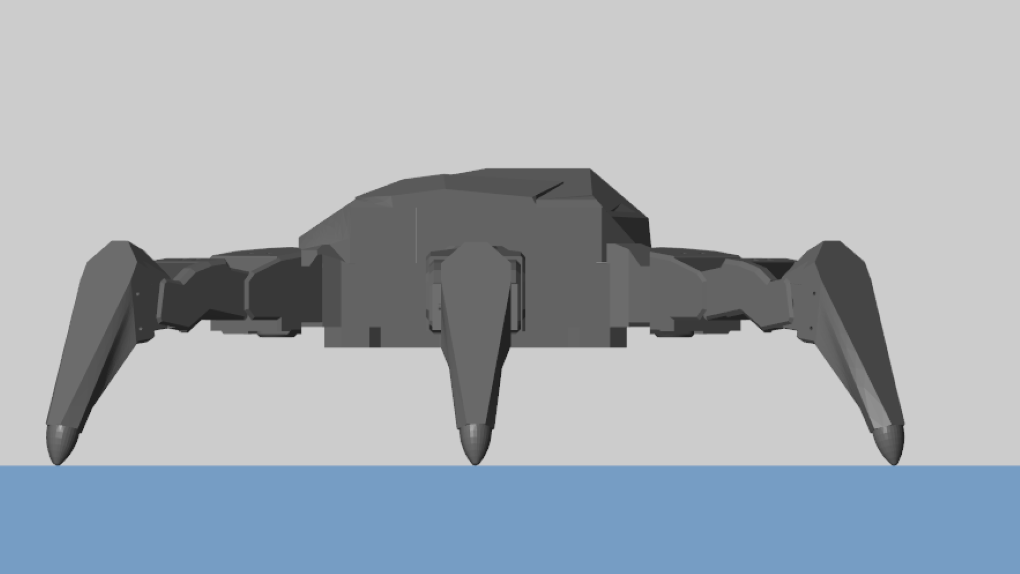
\includegraphics[width=.9\linewidth]{PhantomX_MK4_SideView}  % this sets the image to fill 90% of the available space -> 45% of the line width in total. 
		\caption{}
		\label{figure: PhantomX Side View}
	\end{subfigure}
	\begin{subfigure}{.5\textwidth}
		\centering
		% include second image
		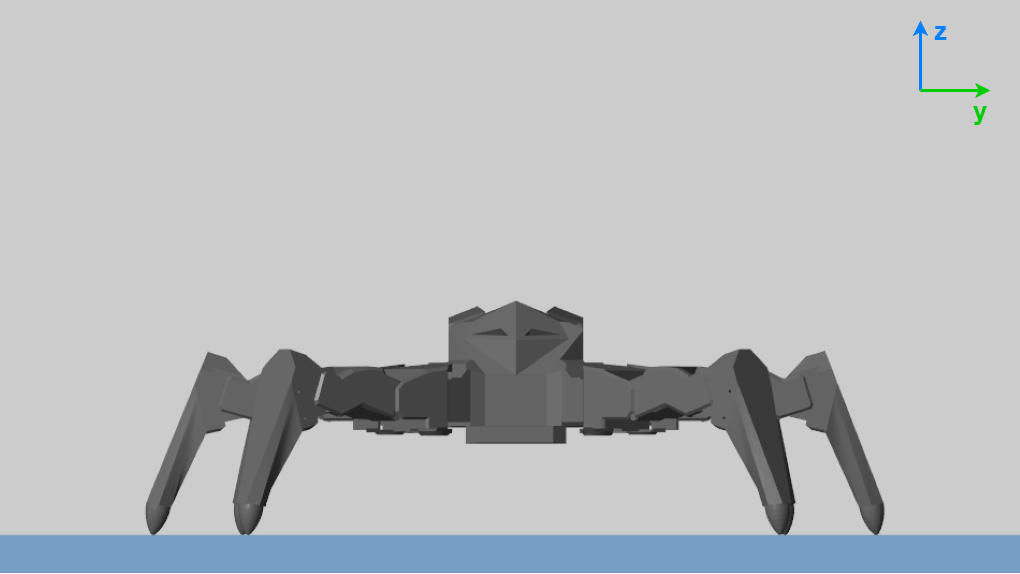
\includegraphics[width=.9\linewidth]{PhantomX_MK4_FrontView}  
		\caption{}
		\label{figure: PhantomX Front View}
	\end{subfigure}
	
	\label{fig:fig}
	\begin{subfigure}{\textwidth}
		\centering
		% include third image
		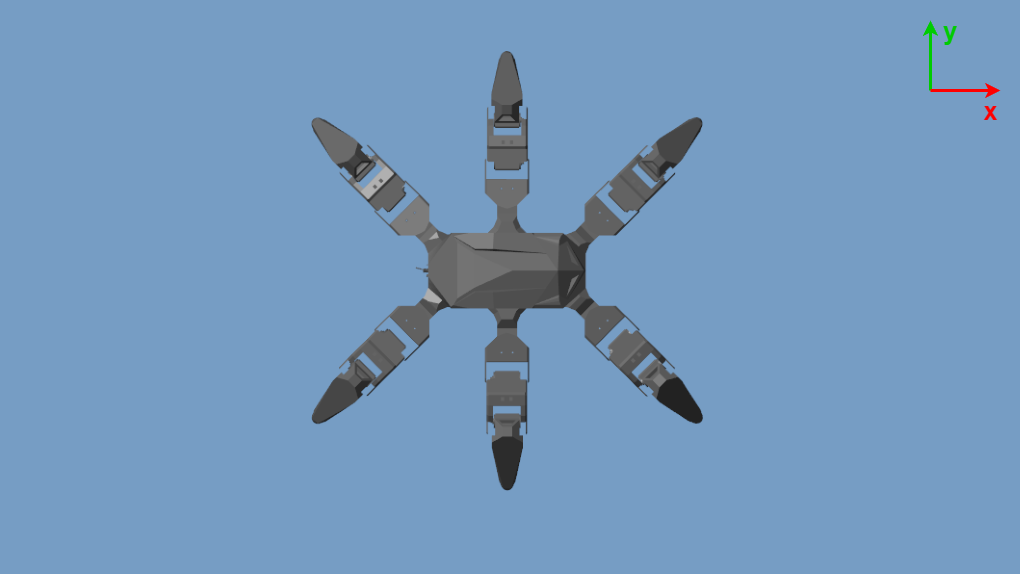
\includegraphics[width=.45\linewidth]{PhantomX_MK4_TopView}   % this width should be half of the width of the other two images
		\caption{}
		\label{figure: PhantomX Top View}
	\end{subfigure}
	\caption[Trossen Robotics PhantomX MKIV]{3D model of Trossen Robotics PhantomX MK4. The central axis $\vec{x}$ can be seen in (a) and (c).}
	\label{figure: PhantomX 3D model}
\end{figure}
\todo{get each image into list of figures, but exclude complete figure}
\todo{add central axis to images}

To be able to use the imported hexapod as a development platform we modify and expand the raw Simulink model as it does not provide any means to exert control over or receive feedback from it.
We reorganise and encapsulate logical groups, specifically the thorax and the individual legs, into library subsystems.
This enables us to propagate changes during the development process faster, as we only have to edit the library component instead of each existing instance.
As a side effect, this compartmentalisation provides the Simulink model with a much more cleaned up and easier to understand appearance.
To be able to control each joint and receive sensory feedback from it, we enable the so called \textit{direct torque input} as well as the \textit{position} and \textit{acceleration} sensor readings on each joint block.
Trying to prevent the models complexity from increasing to quickly, we abstain from modelling the physical servo motor attached to each joint and instead use the instantaneous torque application mentioned above.
The joint block also allows for physical parameters to be modified, such as joint boundaries, internal friction, dampening and spring stiffness.
We combine the 3 torque values and position/ acceleration readings of each leg into an input and output bus signal.
A view inside of the leg subsystem is given in \ref{figure: Hexapod Leg}, the subsystem block itself with its torque input and sensory feedback output buses can be seen in \ref{figure: Hexapod Model Overview} as part of the complete hexapod model.

\begin{figure}[h]
	\centerline{\includesvg[scale=0.55]{Simulink/Simulink_PhysicalHexapodOverview}}
	\caption[Simulink hexapod model overview]{Overview of the Simulink Hexapod Model}
	\label{figure: Hexapod Model Overview}
\end{figure}

\begin{figure}
	\centerline{\includesvg[scale=0.5]{Simulink/Simulink_HexapodLegOverview}}
	\caption[Simulink leg subsystem]{Simulink model of the Hexapod Leg subsystem}
	\label{figure: Hexapod Leg}
\end{figure}

In Simscape, collision modelling involves establishing connections between a rigid body, and any other rigid body it should be able to interact with in a collision scenario, via Simscapes's \textit{Spatial friction force} block.
An example of how the block can be utilized has already been shown in \ref{figure: Simscape Bouncing Ball Example}.
Therefore, to enable the robot to physically interact with its surroundings, we enable the collision geometry on each of the models rigid bodies and connect them over said spatial friction force blocks.
The block allows modifications to collision parameters such as the coefficients of static and dynamic friction, elasticity and dampening.\todo{does dampening exist in block ?}
As collision detection is computationally relative expensive, we refrain from modelling robot self collisions and focus only on the interaction between robot and environment.
The result of this being that the hexapods links can only collide with the ground plane but not with each other.
We realise this can potentially create discrepancies between simulation and real world, but as we only model predefined leg trajectories in this thesis, which can manually be proven to not intersect, we are willing to give up a bit of realism in favour of faster simulations.

The robot model, modified in the ways described, is encapsulated as a single \textit{Hexapod} subsystem block.
It receives the torques to be applied as input and outputs sensory information about each joint.
All of the internal joint parameters and friction coefficients used to model collisions can be modified within the MATLAB-script \textit{simulation\_setup.m} during initialisation of the model.
The parameter values used in all simulations we present in thesis are given in the tables \ref{table: Joint parameters} and \ref{table: Spatial contact force}.
The joint parameter values were already mostly given by the urdf specification, while we adapted most of the friction force parameters from \parencite{trotta2022walking} and \parencite{AUTHOR2}.
\todo{Find source again}
To summarize, we converted the provided hexapod description into a Simulink model, compartmentalized it and added sensing and actuation capabilities to the robots legs.
In addition we made most of the models internal parameters accessible and modifiable within an initialisation script.



\begin{comment}
The  thorax is represented by a rigid body and a main coordinate frame.
Each of the robots legs consists of 3 rigid bodies(coxa, femur and tibia) which are connected to each other by 2 joints.
A third joint then attaches the coxa and the leg as a whole to the main body.
Like the leg of an insect, the movement plane of the joint connecting coxa and thorax is parallel to the ground and orthogonal towards the other two joints.
Each of the joints used has 1 (rotational) DoF.
To position each rigid body and joint correctly, rigid transformations are used to translate and rotate each component.

As mentioned above, joints can receive as input a torque to be applied and can output sensory data, such as the joints position, velocity and acceleration. 
\end{comment}

%In this thesis we only utilize the sensor information about the current joint positions, but to allow for further expansions on the model, such as optimizing for minimal energy consumption, joint velocity and acceleration are provided as well.
%It should be noted, that integrating the joint position over time would implicitly yield the same result, but we decided for ease of use to include this data explicitly.


\subsection{The Environment}
To validate the hexapod model and to provide a space for the robot to learn coordination strategies, we construct a simple test environment.
The environment, at this point, simply consists of a horizontal plane, but can be expanded to include more complex terrain with little effort.
Some examples which we experimented with, but did not utilise for testing or training so far, include inclined planes and small obstacles on the ground.
As Simscape itself only provides basic geometric objects, but allows for the use of .stl files to define the shape of objects, complex terrain such as irregular, uneven surfaces can be imported with relative ease. \todo{check if really .stl and add footnote}
In addition to being the testing ground of the hexapod model, the environment also acts as part of the RL training process.
Similar to the basic concept of RL depicted in Fig. \ref{figure: RL Illustration}, at each time step of the simulation the environment provides RL observations and a reward to the RL agent. \todo{As of now not represented in the model, reward is part of controller}.
In contrast to this basic concept however, the environment as we define it does not directly receive actions from the RL agent.
Instead, the agents actions are applied to the hexapod model, which is its own separate subsystem.
If one would precisely follow the definition of a RL environment in a manner analogous to \ref{figure: RL Illustration}, both the environment subsystem and the hexapod subsystem would have to be included as part of the "RL" environment.
For obvious reasons such as modularity and clarity of model we choose not to adapt this approach.

\subsection{The Locomotion Controller} \label{subsec: Locomotion controller}
As the conductor of the hexapods locomotion, the controller, at a high level of abstraction, sets the speed, gait and direction of the robots movement.
On the lowest operational level, the controller achieves these parameters by precisely controlling the torque applied to each joint at every simulation step.
The locomotion controller subsystem as a whole can be described as a feedback control system.
It receives sensory information about the process it controls (the hexapod robot) and takes this feedback into account when generating new instructions (torque values) to steer the process.
As can be seen in the abstract diagram displayed in Fig. \ref{figure: Controller Overview}, the locomotion controller is comprised of several components. 
In the following, we will explain each of these components (and subcomponents) in detail.

\begin{figure}[h]
	\centerline{\includegraphics[scale=0.03]{HexapodController}}
	\caption[Controller Overview]{Overview of the Locomotion controller}
	\label{figure: Controller Overview}
\end{figure}

As the robots legs have to be able to move independently from one another, the controller contains 6 separate \textit{control units}, one for each of the six legs.
These units receive sensory information from the leg's \textalpha-joint, more precisely the position and acceleration readings, as input and compute the torques to be applied to them as output.
In addition, each leg control unit receives the desired frequency of the swing-stance cycle $f_{c}$, the duty-cycle percentage $P_{swing}$ and the swing-initiation signal of the respective leg $s_i,\ i \in \{1,...,6\}$ as coordination inputs.\todo{Explain why we use a Initiation Signal -> RL}
The frequency $f_{c}$ defines how often the swing-stance cycle should be repeated per second, $f_{c} = 0.5 \text{ Hz}$ for example corresponding to one full cycle every 2 seconds.
$P_{swing}$ defines the proportion of the swing (duty) phase in relation to a whole cycle \parencite{qiu2023adaptive} and can be expressed by: 

\begin{equation}
P_{swing} = \frac{T_\text{sw}} {T_\text{st} + T_\text{sw}}
\end{equation}
where $T_\text{sw}$ and $T_\text{st}$ are the durations of the swing and stance phase respectively, given as:
\begin{equation}
T_\text{sw} = \frac{P_\text{swing}}{f_c}, \quad T_\text{st} = \frac{1-P_\text{swing}}{f_c}
\end{equation}

A 50\% duty cycle ($P_{\text{swing}} = 0.5$) results in swing and stance being of equal length, both taking up exactly half a cycle time.
The swing initiation signal $s_i \in \{0,1\}$ for each of the six legs ($i \in \{1,...,6\}$) indicates to the control unit whether to initiate the swing phase ($s_i = 1$), independent of the legs position in the cycle, or whether to continue on with the current cycle execution ($s_i = 0$).
The control units also receive a movement direction vector $\vec{d}$ as an additional input.
All of the inputs can either be received from a \textit{Static Gait Definition}, in which the parameters are configured prior to simulation, or can be provided by a RL agent.

The \textit{Simulink RL Agent}, a standard library block and separate component in the controller subsystem, receives the observations $\vec{o_t}$ from the hexapod model as well as a reward signal $r(t)$ at each time step.\todo{Make distinction between observations an RL data, which also includes information about the reward}
It outputs an action vector $\vec{a_t} = (s_1,...,s_6)$, which consists of the swing initiation signal for each leg.
To reduce complexity, we restrict agents to control over these $s_i \in \{0,1\},\ i \in \{1,...,6\}$, while all other parameters stay fixed during a simulation run.
The RL agent block belongs to the \textit{Reinforcement Learning} library and represents an agent in the same sense as described in \ref{sec: Reinforcement Learning}.
Further and more detailed elaboration on both RL agent and reward function will be provided in section \ref{sec: RL setup}.

\begin{figure}
	\centerline{\includesvg[scale=0.6]{Simulink/Simulink_LegControllerOverview}}
	\caption[Single leg control unit]{Control unit for a single leg}
	\label{figure: Leg control unit}
\end{figure}

Continuing  with the description of the locomotion controller, we focus on a single leg control unit.
Such a unit, as shown in Fig. \ref{figure: Leg control unit}, consists of a \textit{Leg Trajectory Generator} and three PID feedback control loops, one for each joint.
The leg trajectory generator is responsible for providing the joint angles required to allow the leg's end-effector to follow a smooth trajectory, all in accordance to $f_c$, $P_\text{swing}$, $s_i\ (i \in \{1,...,6\})$ and $\vec{d}$.
At each time step, the generator calculates the angles of the \textalpha-, \textbeta- and \textgamma-joint, which are send to the PID controllers to be used a their new setpoints.
The PID controllers then work on achieving the desired angles by regulating the applied torques.
The PID parameters $K_p$, $K_i$, $K_d$ (and $N$) are tuned via trial-and-error method and are given in table \ref{table: PID parameters}.
\todo{This section might need a rewrite for better formulation}

\begin{figure}
	\centerline{\includesvg[scale=0.75]{Simulink/Simulink_LegTrajectoryGenerationOverview}}
	\caption[Leg Trajectory Generator]{Leg trajectory generator}
	\label{figure: Leg trajectory generator}
\end{figure}

Moving down another level of complexity, the leg trajectory generator, as seen in Fig. \ref{figure: Leg trajectory generator}, consists of a \textit{Signal Generator}, a \textit{Pattern Rotation} subsystem and an \textit{Analytical IK Solver}.
The signal generator is responsible for the generation of a continuous leg trajectory in the form of 2-dimensional trajectory coordinates.
We provide insights into the exact process of coordinate signal generation in the upcoming section.
As we intent the locomotion controller to allow for omnidirectional movement, the pattern rotation subsystems applies a simple mathematical rotation to the planar trajectory (x,z-plane) around the z-axis.\todo{Introduce coordinate system at the beginning of methods}
The required rotation angle is determined from the angle between the default forward movement direction $\vec{d}_\text{default} = (1 \ 0 \ 0)^t$ and $\vec{d}$.
Finalizing the trajectory generator, the analytical IK solver receives the calculated trajectory coordinates and translates them into the \textalpha, \textbeta \ and \textgamma \ joint angles.
A more detailed explanation of the solver is provided in \ref{subsubsec: IK Solver}.


\todo{Remove text from image/ change image to diagram}
\todo{Redo section about Signal Generator after image is refreshed}
The Signal Generator, displayed in Fig. \ref{figure: Signal Generator}, consists mainly of two components, a \textit{Swing Phase} subsystem and a \textit{Stance Phase} subsystem.
These provide the 2-dimensional trajectory coordinates (x,z) during their respective phases in the movement cycle.
Coordination between the two units is achieved through the so called \textit{Swing-Stance Activation} subsystem and is influenced by $f_c$, \ $P_{swing}$ and $s_i,\ i \in \{1,...,6\}$.
If $s_i$ is pulled high ($s_i=1$), the swing phase subsystem is reset and the outputs (x,z) are switched to this system.
In Simulink, resetting a subsystem means the current state of the subsystem is discarded and it's initial state recreated.
At the conclusion of the leg's swing phase (the x-coordinate coincides with the AEP), the swing phase subsystem gives up control to the stance phase subsystem via the \textit{Swing finished} signal.
This act induces a reset on the stance phase subsystem and switches the outputs over to this system.
\\
In detail, the swing and stance phase trajectory coordinates are generated by modulation of geometric and linear functions based on $f_c$, $P_{swing}$ and the function amplitudes.
These amplitudes are derived from the desired step length and height.
The swing trajectory $\Theta_{sw}(t)$ and the stance trajectory $\Theta_{st}(t)$ are defined as follows:
\begin{align}
	\Theta_{sw}(t) & = 
	\begin{cases}
		x_{sw}(t) = x_{st} + \frac{|AEP - x_{st}|}{2} \cdot \cos(f_{sw} \cdot t \cdot \pi + \pi) + \frac{|AEP - x_{st}|}{2} \\
		z_{sw}(t) = h_{step} \cdot \sin(f_{sw} \cdot t \cdot \pi) \\
	\end{cases} & , t \in [0,T_\text{sw}] \\
	\notag \\
	\Theta_{st}(t) & =
	\begin{cases}
		x_{st}(t) = \text{AEP} - f_{st} \cdot t \cdot l_{step}\\
		z_{st}(t) = 0
	\end{cases} & , t \in [0, T_\text{st}]    
\end{align}
We define $l_{step} = |AEP - PEP|$ as the length of a step, $h_{step}$ as the predefined height of a step and $x_{st}$ as the x-coordinate of the leg at the moment the swing phase is initiated.
Given $f_c$ and $P_{swing}$, we further define $f_{sw} = \frac{f_c}{P_{swing}}$ and $f_{st} = \frac{f_c}{1-P_{swing}}$ as the frequency of the swing and stance phase respectively.
The parameter $t$ is limited to the ranges $[0,T_\text{sw}]$ and $[0, T_\text{st}]$, as every time one of the subsystems reaches the end of its phase ($t=T_{sw}$ or $t=T_{st}$), the subsystems internal clock is reset and upon it's next activation, the function evaluation starts at $t=0$ again.

\todo{Double-check equations}
\todo{Insert image of trajectory graphs/ create graphic depicting early swing initiation and resulting trajectory}

\begin{figure}[!h]
	\centerline{\includesvg[scale=0.75]{Simulink/Simulink_SignalGeneratorOverview}}
	\caption[Signal Generator]{Signal Generator}
	\label{figure: Signal Generator}
\end{figure}

\begin{figure}[!h]
	\centerline{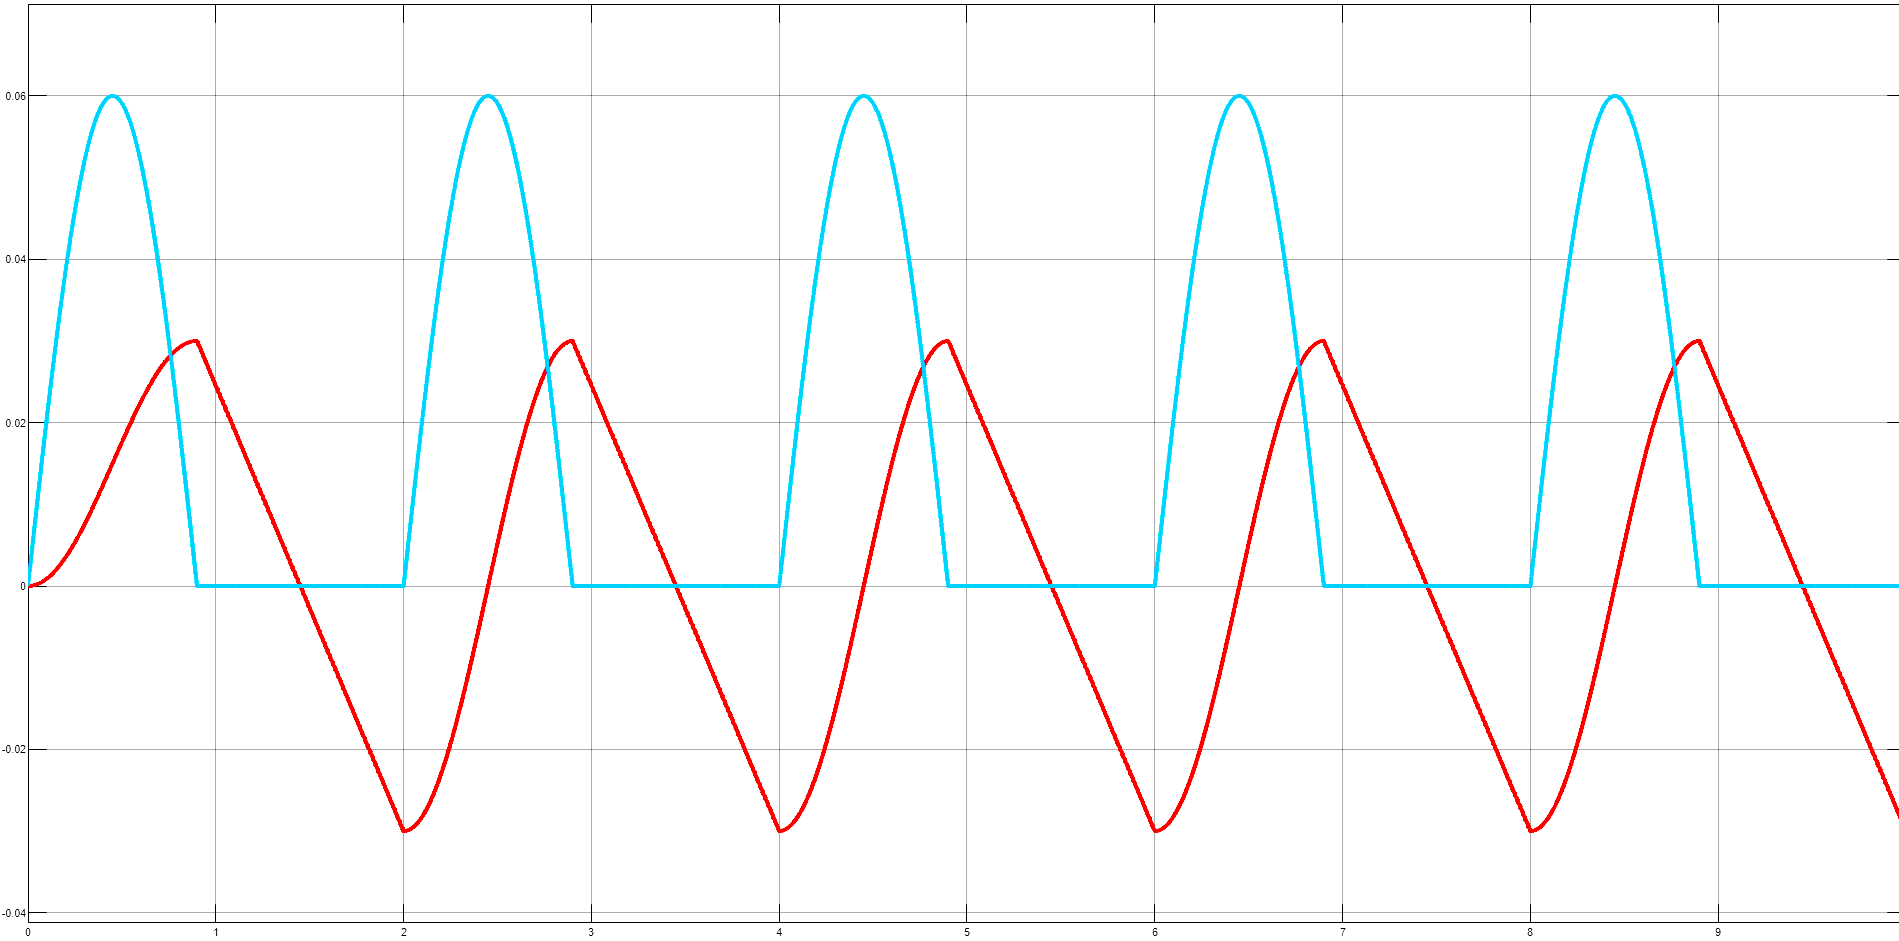
\includegraphics[scale=0.2]{Simulink/SignalGenerator_Graph_0.5Hz.PNG}}
	\caption[2D Trajectory Coordinates]{Trajectory coordinates generated by a signal generator with $f_c=0.5$\ Hz, $P_{Swing}=40\text{\%}$}
	\label{figure: Trajectory graphs}
\end{figure}

\begin{figure}[!h]
	\centering
	\begin{subfigure}[b]{0.55\textwidth}
		\includesvg[width=1\linewidth]{Simulink/Simulink_SwingPhaseGenOverview}
		\caption{}
		\label{fig:Ng1} 
	\end{subfigure}
	
	\begin{subfigure}[b]{0.55\textwidth}
	%	\includesvg[width=1\linewidth]{Simulink/Simulink_SwingPhaseGenOverview}
	\includegraphics[scale=0.5]{example-image-b}
		\caption{}
		\label{fig:Ng2}
	\end{subfigure}
	
	\caption[Swing and Stance Phase]{(a) Swing phase subsystem. The swing ellipse is generated by two sine waves with different amplitude and phase. (b) Stance phase subsystem. As opposed to (a), the x-coordinate is now generated by a linear function and the z-coordinate is 0 throughout the whole phase.}
\end{figure}


\subsubsection{Analytical Inverse Kinematics Solver} \label{subsubsec: IK Solver}
While Simulink's \textit{Robotics System Toolbox} does provide an iterative IK block, it is unable to support the calculation speed we require.
To achieve stable simulations and smooth motion of the hexapod robot, the model requires a simulation step-size of about 0.5 ms, equating to a trajectory calculation frequency of 2 kHz.
At this compute frequency, the provided iterative solver becomes a bottleneck in the simulation cycle, resulting in unacceptable simulation times.
To drastically reduce the computation time a simulation step requires, we implement our own, purpose-build analytical IK solver.

\begin{figure}[!h]
	\begin{subfigure}{.5\textwidth} % this sets the figure to be max half the width of the page
		\centering
		% include first image
		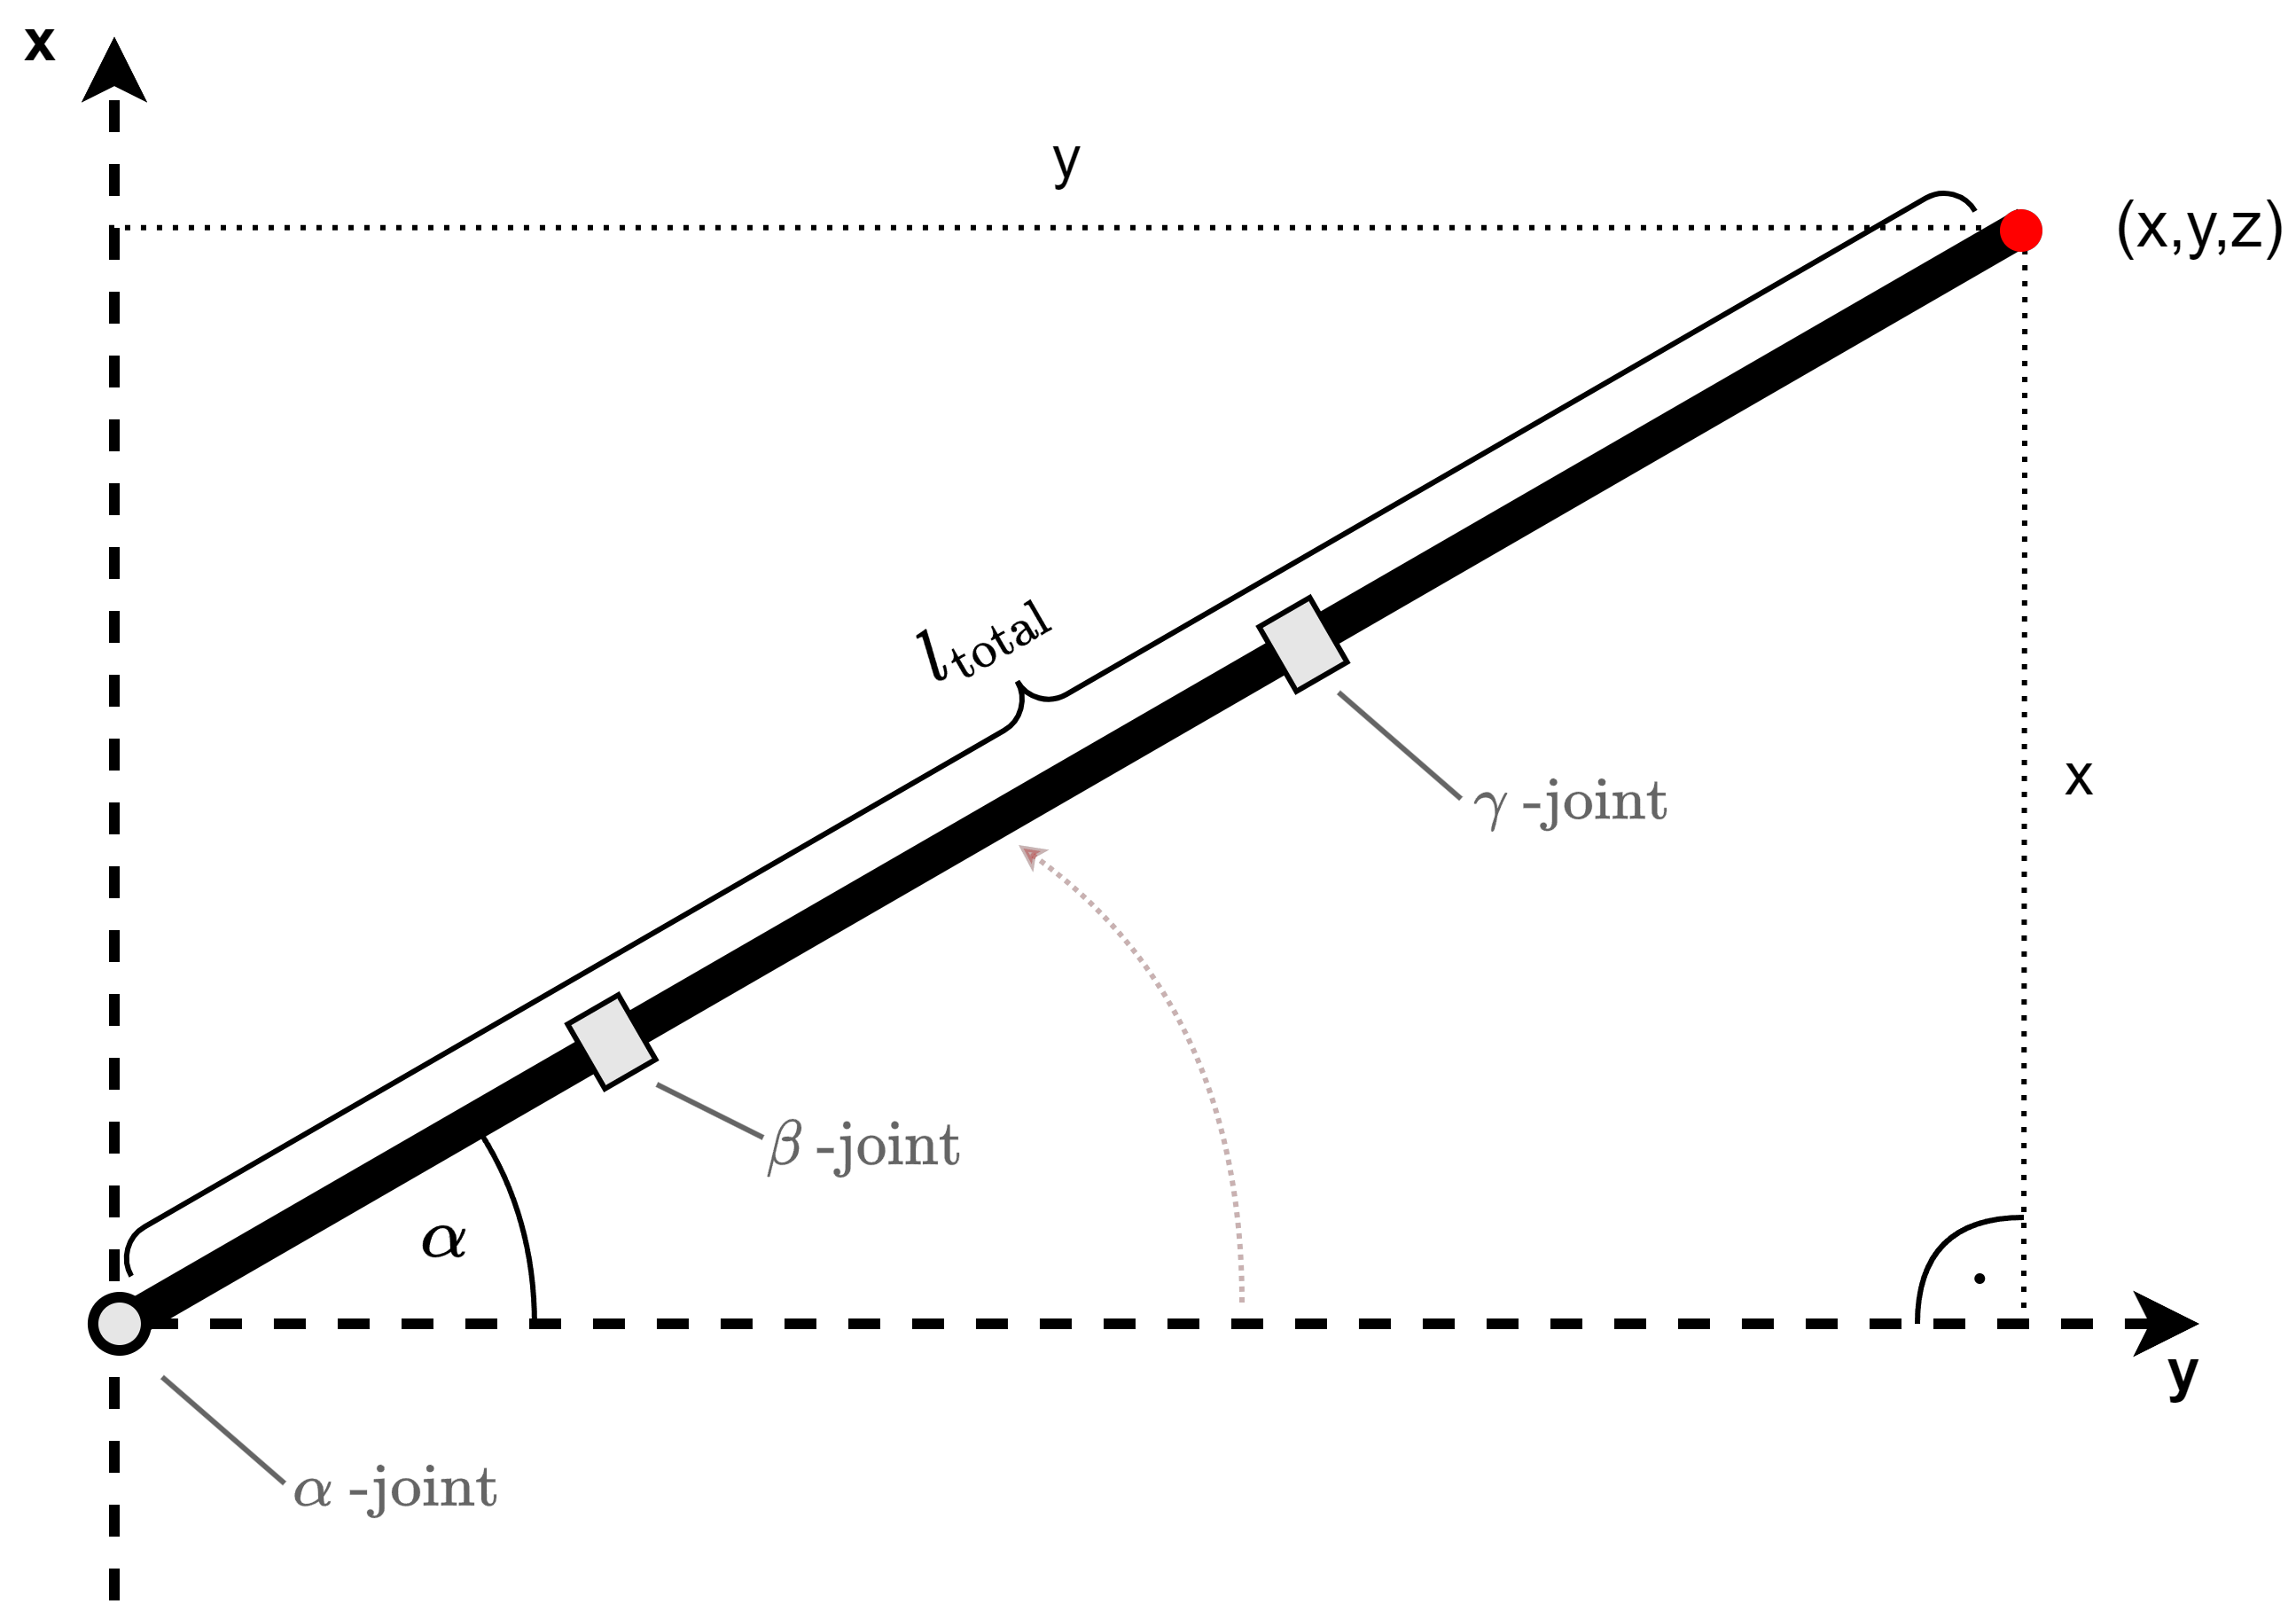
\includegraphics[width=\linewidth]{IK_Solver_alphaAngle}  % this sets the image to fill 90% of the available space -> 45% of the line width in total. 
		\caption{}
		\label{figure: IK Solver Alpha Angle}
	\end{subfigure}
	\begin{subfigure}{.5\textwidth}
		\centering
		% include second image
		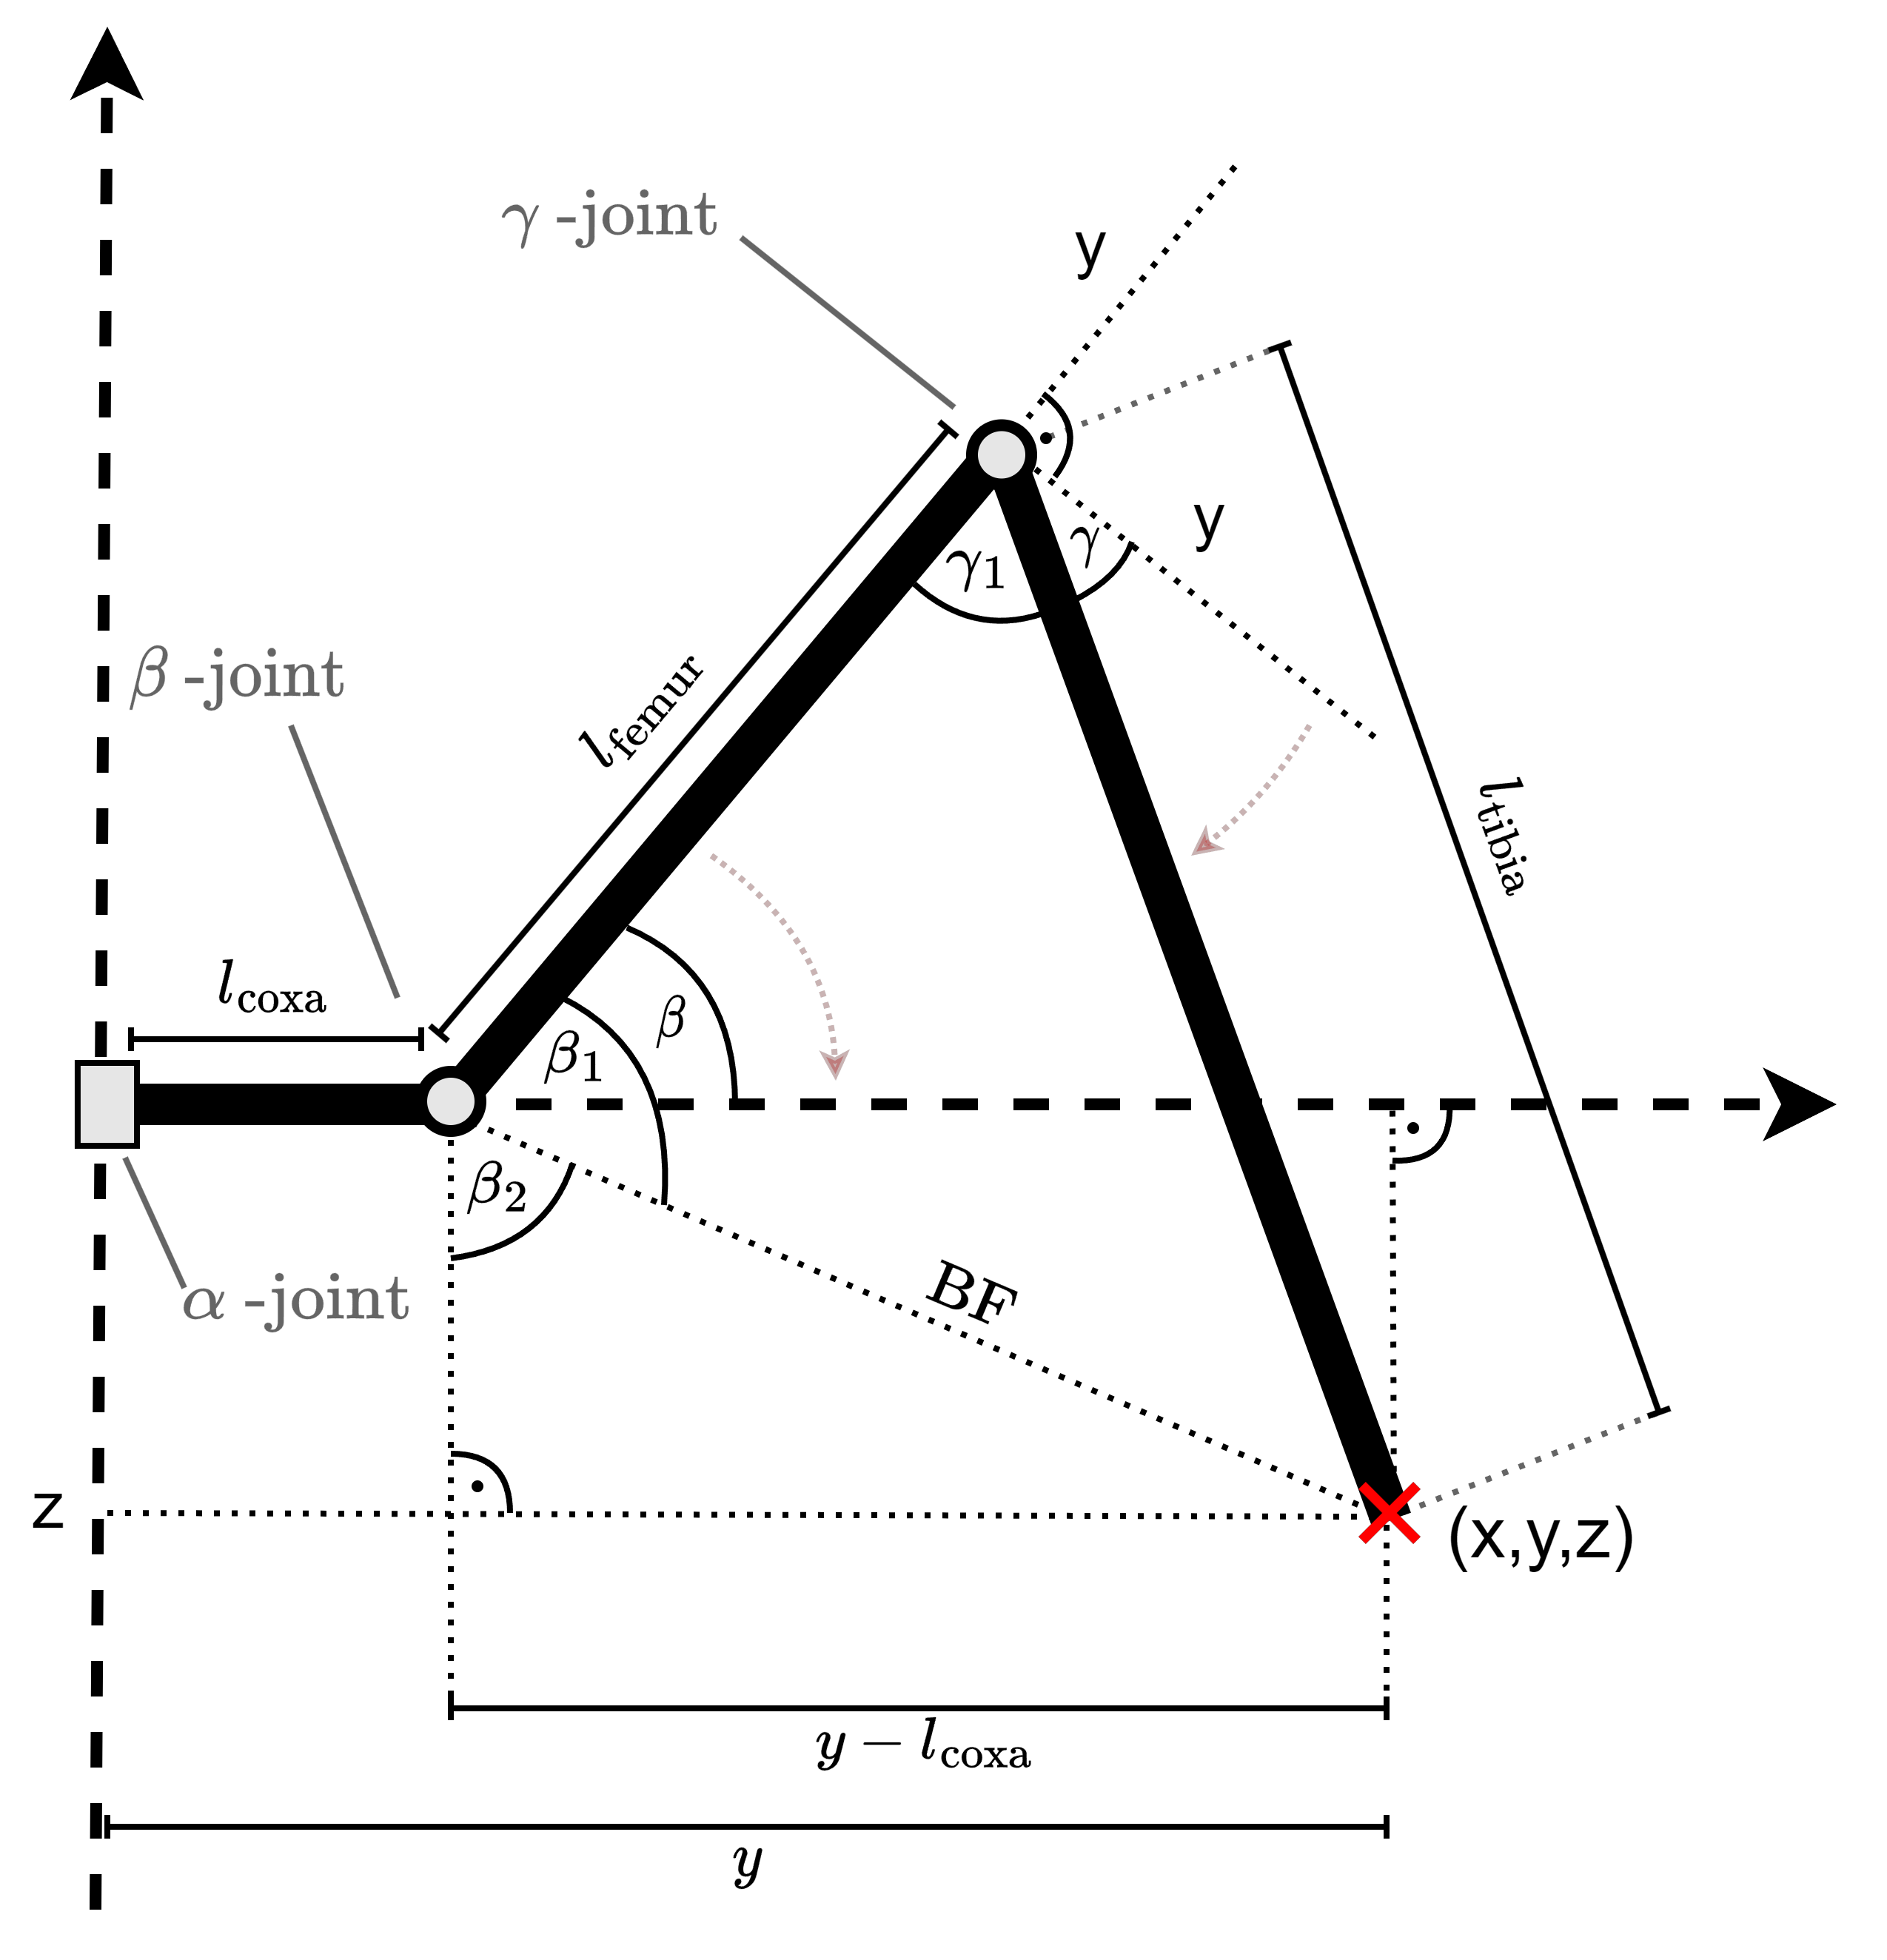
\includegraphics[width=0.85\linewidth]{IK_Solver_betaGammaAngle}  
		\caption{}
		\label{figure: IK Solver Beta/Gamma Angle}
	\end{subfigure}
	\caption[Angle derivation drawings]{(a) Top-down view of a hexapod leg, used to determine \textalpha. (b) Side-view, used to calculate \textbeta \ and \textgamma.}
	\label{figure: IK angle derivations}
\end{figure}


\begin{figure}[!h]
	\begin{subfigure}{.5\textwidth}
		\centering
		% include second image
		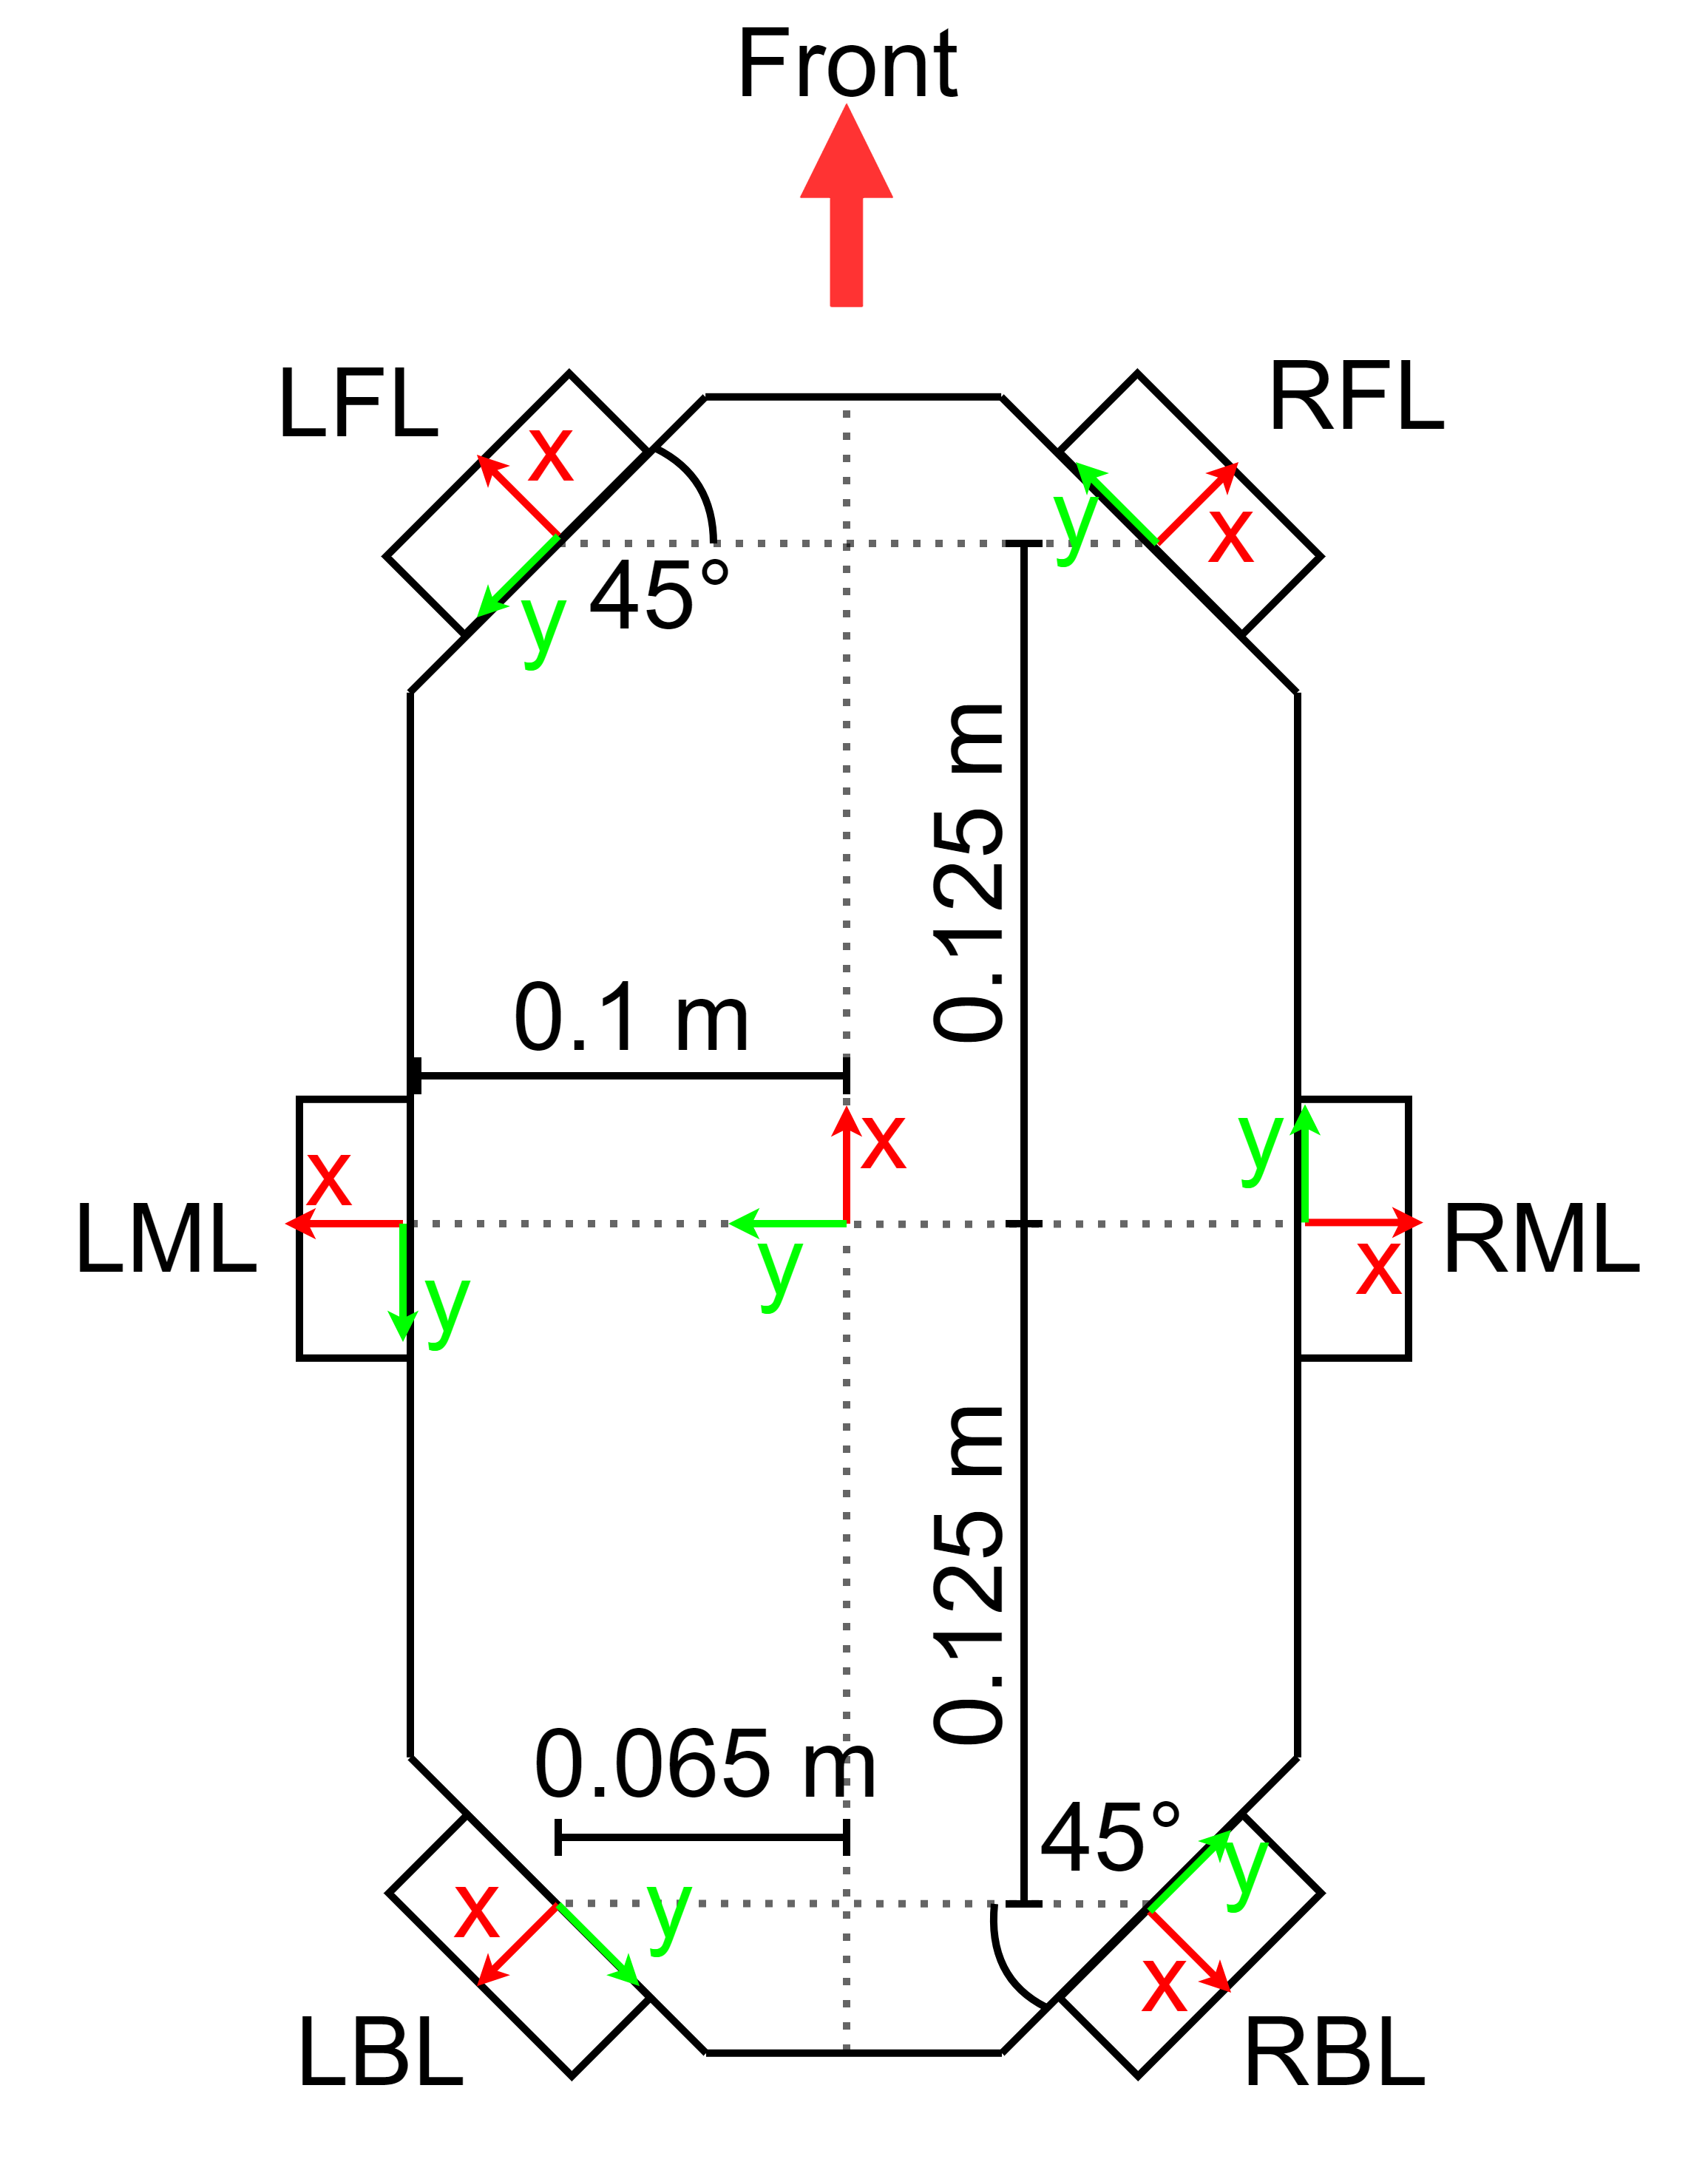
\includegraphics[width=\linewidth]{Hexapod_Offsets_Sketch.png}  
		\caption{}
		\label{figure: Hexapod thorax sketch}
	\end{subfigure}
	\begin{subfigure}{.5\textwidth} % this sets the figure to be max half the width of the page
		\centering
		% include first image
		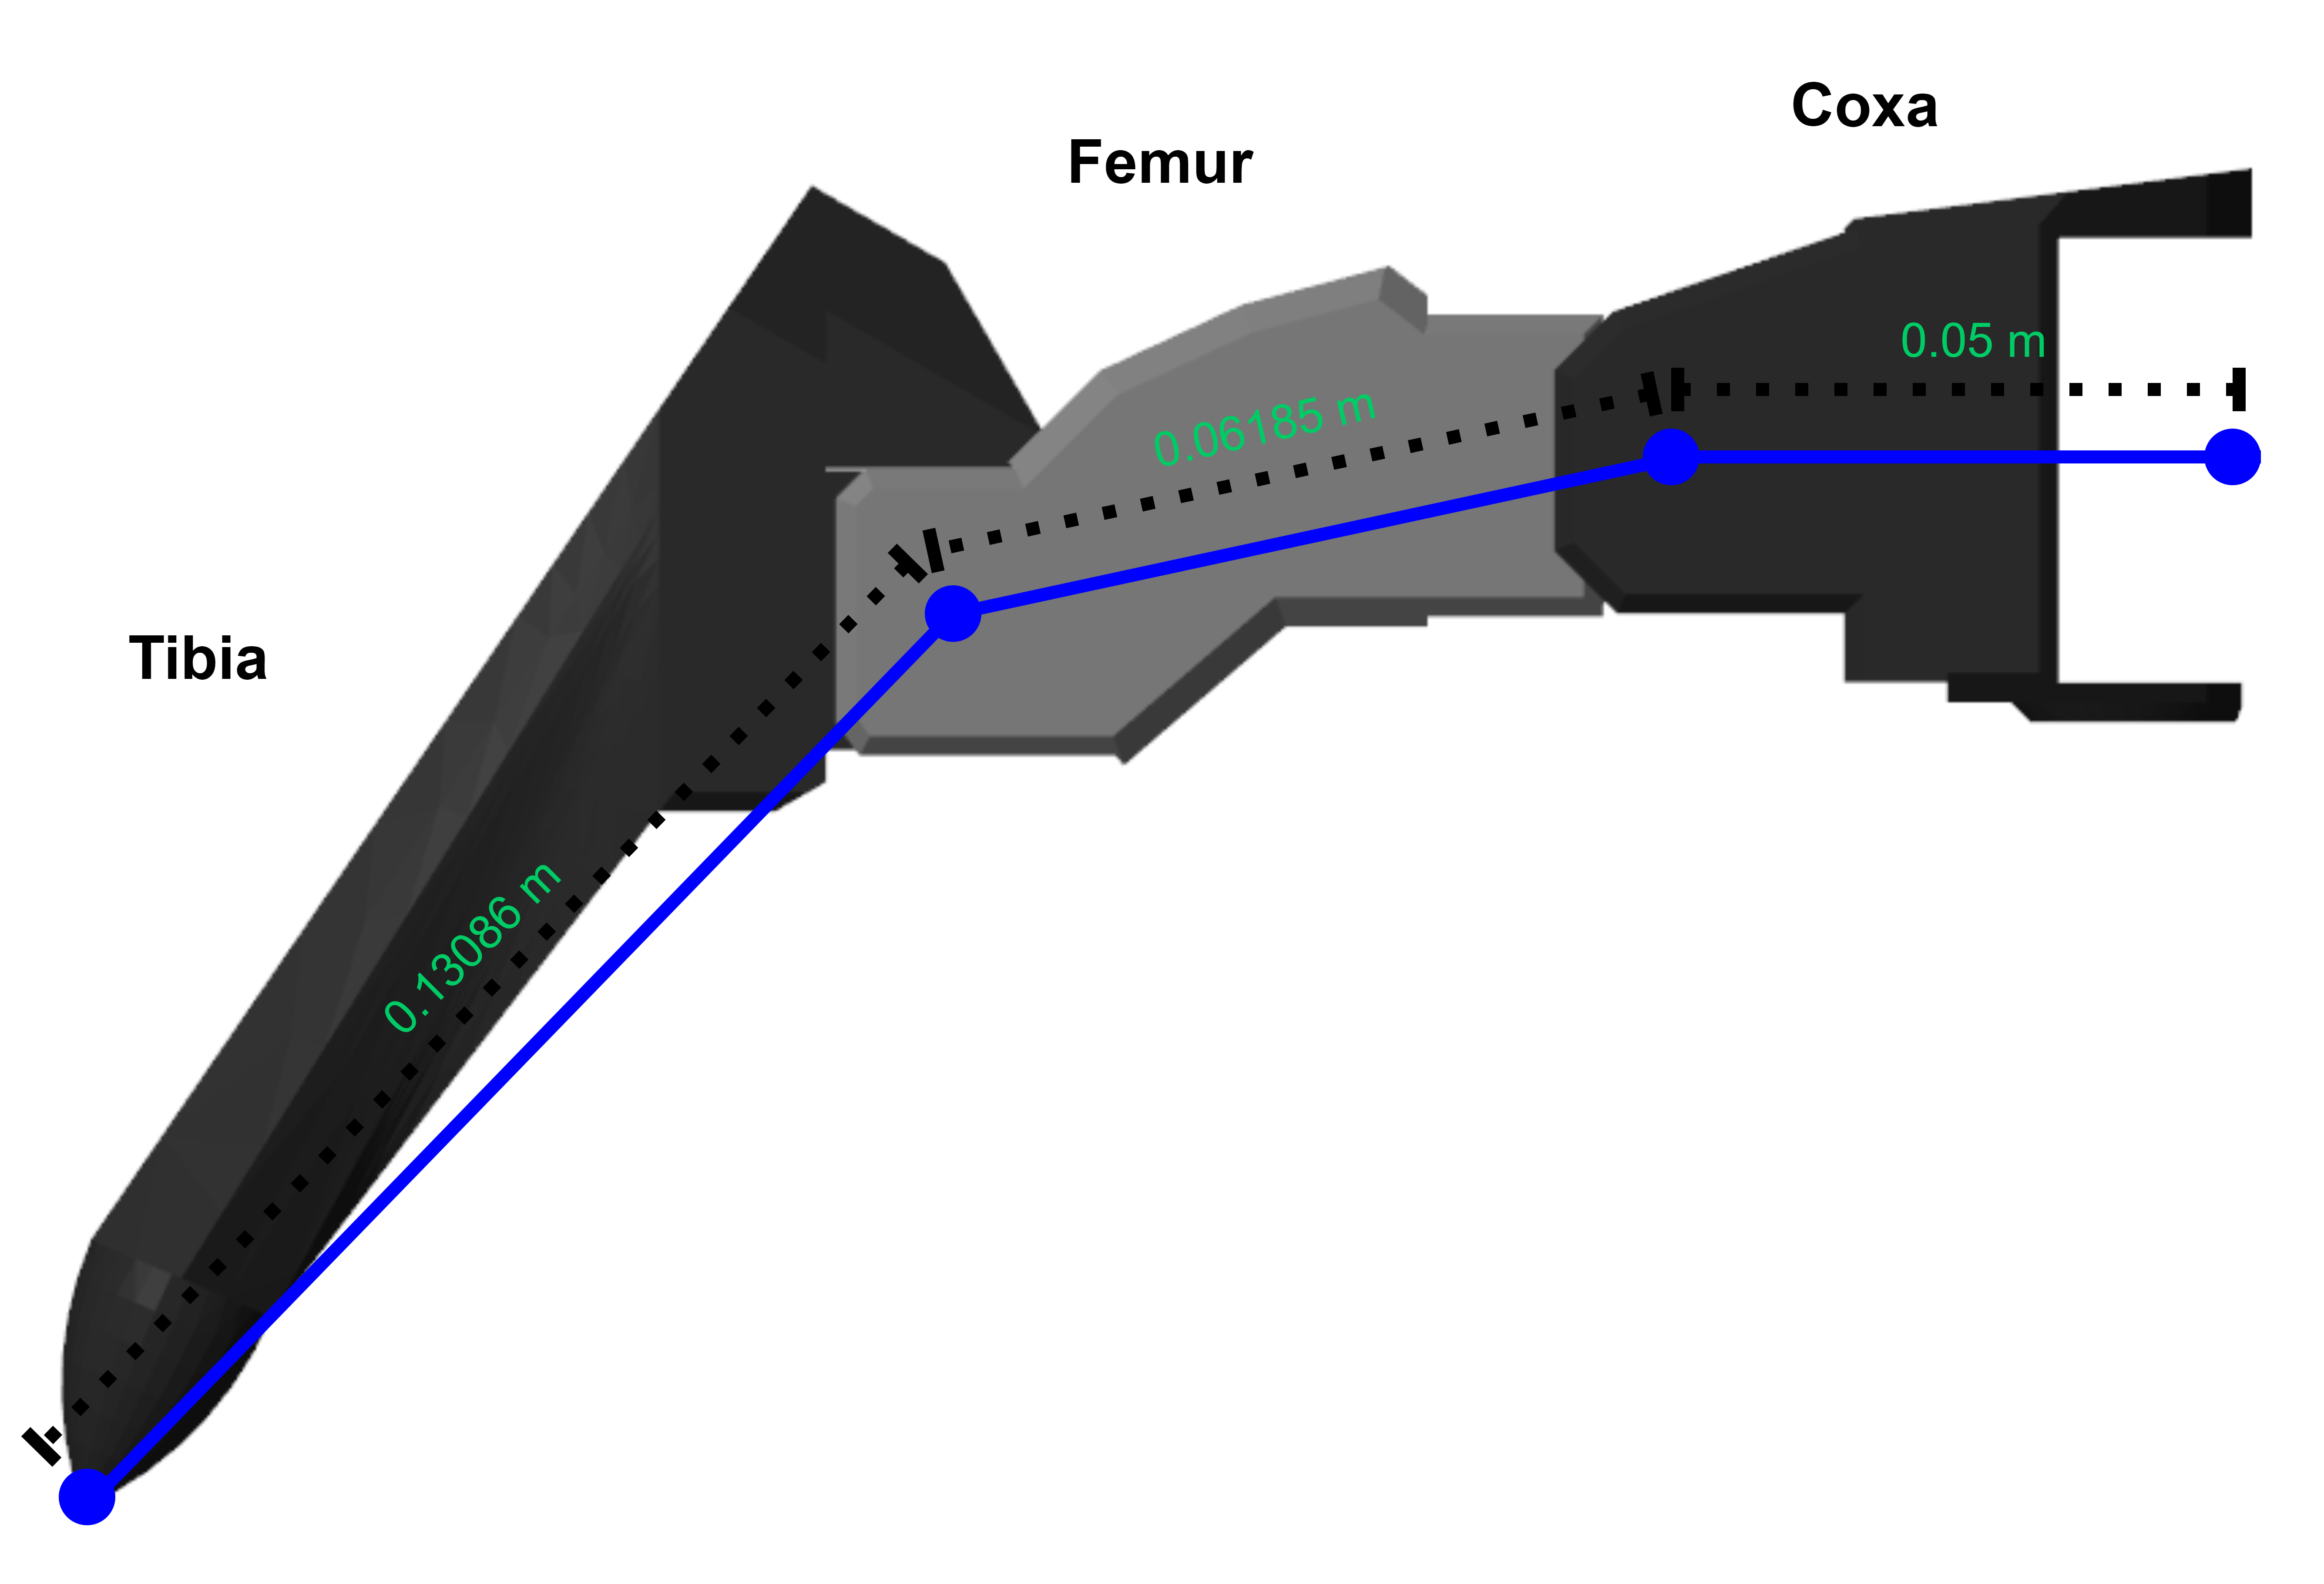
\includegraphics[angle=-90,width=0.8\linewidth]{HexapodLeg_Lengths.PNG}  % this sets the image to fill 90% of the available space -> 45% of the line width in total. 
		\caption{}
		\label{figure: Hexapod Leg proportions}
	\end{subfigure}
	\caption[Hexapod proportions]{(a) Drawing of the PhantomX MK4 thorax, annotated with proportions. (b)  Leg segment proportions of the PhantomX MK4 hexapod legs.}
	\label{figure: Hexapod proportions}
\end{figure}
\todo{Increase fontsize}

Our proposed solver sequentially calculates the legs joint angles, starting at \textalpha, then \textbeta \ and \textgamma.
We derive the following equations from the geometric properties of a hexapod leg as seen in \ref{figure: IK angle derivations}:

\[
	\alpha = \arctan(\frac{x}{y}) ,\quad \quad \quad \beta = 90^{\circ} - (\beta_1 + \beta_2) ,\quad \quad \quad \gamma = 90^{\circ} - \gamma_1.
\]
\\
Where $\beta_1$, $\beta_2$, $\gamma_1$ and \text{BF} are given by:
\[	
	\beta_1 = \arccos(\frac{{l_\text{femur}}^2 + \text{BF}^2 - {l_\text{tibia}}^2}  {2\cdot l_\text{femur} \cdot \text{BF}}) ,\quad \quad \quad \beta_2 = \arctan(\frac{ l_\text{total} - l_\text{coxa}} {z}),
\]

\[
	\gamma_1 = \arccos(\frac{{l_\text{tibia}}^2 + {l_\text{femur}}^2 - {\text{BF}}^2}  {2 \cdot {l_\text{tibia}} \cdot {l_\text{femur}}}) ,\quad \quad \quad \text{BF} = \sqrt{(l_\text{total} - l_\text{coxa})^2 + z^2}.
\]

To create the Analytical IK block, we translate the derived equations into C-code.
The implemented code (\textit{InverseKinematics.c}) is then run inside a \textit{MATLAB code block} for each simulation step.
As the hexapods initial joint positions deviate from the ones displayed in Fig. \ref{figure: IK angle derivations}, we require the offsets to convert the angles calculated by the solver to match these differing initial positions.
The offsets are given in table \ref{table:Joint position offsets}.


\section{Learning Leg Coordination} \label{sec: RL setup}
\todo{Redo this section}
From a RL point of view, the leg coordination problem can be considered a POMDP (Partially observable Markov decision process).
The POMDP is an extension to the MDP definition and describes problem spaces in which only parts of the environment can be observed.
This is particularly the case for complex, continuous environments in which it is impossible to observe every environmental detail.
For the problem we attempt to solve, this holds true as well.

\begin{definition}[Partially Observable Markov Decision Process {[\cite{silver2015}]}]
	A \textbf{POMDP} is a 7-tuple $\langle \mathcal{S,A,O,P,R,Z,\gamma} \rangle$
	\begin{itemize}
		\item $\mathcal{S}$ is a set of states
		\item $\mathcal{A}$ is a finite set of actions
		\item $\mathcal{O}$ is a finite set of observations
		\item $\mathcal{P}$ is a state transition probability matrix, $\mathcal{P}_{ss'}^a = \mathbb{P}[S_{t+1} = s' \ | \ S_t = s, A_t = a	] $
		\item $\mathcal{R}$ is a reward function, $\mathcal{R}_s^a = \mathbb{E}[R_{t+1} \ | \ S_t = s, A_t = a]$
		\item $\mathcal{Z}$ is an observation function, $\mathcal{Z}_{s'o}^a = \mathcal{P}[O_{t+1} = o \ | \ S_{t+1} = s', A_t = a]$
		\item $\mathcal{\gamma}$ is a discount factor $\mathcal{\gamma} \in [0,1]$
	\end{itemize}
\end{definition}

In the following, we will describe our RL setup in terms of a POMDP:\\
Our state space $\mathcal{S}$ consists of all possible configurations of the hexapod robot and environment.
The action space $\mathcal{A}$ is defined as the set of all possible actions the RL agent can take, namely the decisions on whether to initiate a legs swing phase or not.
The observation space $\mathcal{O}$ consists of the position and acceleration reading om each of the robots 6 \textalpha-joints, totalling 12 observations.
% permutations of the action tuple $\{s_1,...,s_6\}$, meaning it is the set of all 6-bit binary numbers and thus is of size $2^6$.
%It follows that the action space is discrete, as the agent can only decide to activate a swing phase or not.\\
As they are not required for the training process, we do not go into further detail about the state transition probability matrix $\mathcal{P}$ or observation function $\mathcal{Z}$.
The reward function $\mathcal{R}$ given by:
 \[
 R(t) = c_{s_x} \cdot s_x(t) + c_{v_x} \cdot v_x(t) - c_{v_y} \cdot v_y(t) - c \cdot \Delta_\text{h}(t) - c_{W} \cdot W(t) \ + r_\text{survival}.
 \]
 
The components of the reward function are:
The distance $s_x(t)$ and speed $v_x(t)$ the robot reaches along the x-axis, the speed $v_y(t)$ along the y-axis with which the robot deviates from its straight path, the difference between the robots current height and the desired height $\Delta_\text{h}(t)$, the energy consumption $W(t)$ and the survival reward $r_\text{survival}$.
By negatively rewarding height differences during movement of the hexapod as well as energy consumption, we aim to prevent undesirable jumping or twitching behaviour.
By rewarding the agent for its survival time ($r_{survival}$), we aim to provide an incentive for the agent to abstain from terminating the simulation episodes prematurely.
We experiment with several different discount factor $\gamma$, see chapter \ref{ch:results} for more information.
Details about the weights $c_{s_x}, c_{v_x}, c_{v_y}, c_{v_y}, c_{W}$ will be provided in chapter \ref{ch:results}.

As some behavioural patterns of the agent can immediately be determined to be undesirable, such as jumping, not moving at all or deviation to far from a straight line, we terminate episodes displaying this behaviour.
More precisely, the termination criteria are:
\begin{enumerate}
	\item \textbf{Jumping}: The average height of the robots \textalpha-joints is above a certain maximum
	\item \textbf{Inactivity}: The robot did not exceed a speed of $\num{5e-3}\frac{cm}{s}$ over a timespan of 1 second
	\item \textbf{Deviation}: The total deviation on the y-axis is greater than 20 cm
\end{enumerate}

As policy optimization methods, we choose to use both the DDPG (Deep Deterministic Policy Gradient) and PPO (Proximal Policy Optimization) algorithms, as they have already proven themselves to work well in tasks concerning robotic locomotion\parencite{FIND AUTHOR}.\todo{Find authors who used DDPG and PPO for robotics(PPO bei Schilling et al.(?), DDPG bei ? )}
To use agents based on these algorithms in combination with a Simulink model, the model needs to include a \textit{RL agent} block from the \textit{Reinforcement Learning} toolbox.
We also define an observation and action space as well as an environment object in the MATLAB Workspace.
%There are 2 options for agent creation: The \textit{Reinforcement Learning Designer} MATLAB app with a reduced graphical interface or a MATLAB script-file in which the agent is defined in detail.
We choose the utilize MATLAB scripts for this purpose, as this allows us to permanently specify agents and automate the agent setup task.
For each of the agents, DDPG and PPO, we write a separate initialization script.

To speed up the learning process, we decide to utilize \textit{MATLABs Parallel Computing} toolbox.
The toolbox allows us to initialize a parallel pool of several workers, each of whom runs a separate episode of the RL training process.
The parallel learning process is carried out asynchronously, meaning workers that conclude an episode of training do not have to wait on the other workers to finish as well before proceeding.
In contrast to synchronous parallelization, in which the workers send their results to the parallel pool client all at the same time, receiving updates to their parameters all at once, workers under asynchronous parallelization can send their results as soon as their episode terminates and instantly receive parameter updates.
%By parallelization, we significantly improve the number of simulated episodes.

We start the training of agents at a relatively small simulation step size(0.00025s = 0.25ms) to prevent simulation errors due to initial random jerking of robot legs.
After the agent has stabilized, the step size is increased to speed up the further learning process.
\cite{lillicrap2015continuous}

\section{Model Parameters}
In this last section of the methods chapter, we provide the parameters used in various components of the Simulink model.

The internal joint parameters are included in the hexapod .urdf-file and were automatically imported.
We adapted these parameters provided by \textit{Trossen Robotics} \parencite{interboticsGithub} almost completely, changing only the \textit{Transition Region Width}.
The transition region defines a buffer around the joints boundaries, in which the boundaries spring and damping forces act upon the joint.
The smaller the transition region, the sharper the sharper the onset of forces upon the joint and the smaller the required simulation time-step.
We  therefore change the transition region width from  from 0.1° to 1°, sacrificing a small amount of simulation accuracy for an increase in simulation speed.

{\def\arraystretch{1.4}\tabcolsep=5pt
	\begin{table}[!h]
		\centering
		\begin{tabular}{| l | c | c |}
			\hline
			\textbf{Parameter} & \textbf{Value} & \textbf{Unit}\\
			\hline
			\hline
			Spring stiffness & 0 & $\frac{Nm}{\text{deg}}$\\
			
			Damping & 0 &  $\frac{\text{kg} \cdot m^2}{\text{rad} \cdot s}$\\
			
			Spring stiffness (joint boundary) & \num{1e-4} & $\frac{Nm}{\text{deg}}$ \\
			
			Damping coefficient (joint boundary) &  10 & $\frac{Nm \cdot s}{\text{deg}}$\\
			
			Transit region width (joint boundary) & 1 &  deg\\
			\hline
		\end{tabular}
		
		\caption{Internal joint parameters}
		\label{table: Joint parameters}
	\end{table}
}

\todo{"Gait Self-learning for Damaged Robots Combining Bionic Inspiration and Deep Reinforcement Learning" for parameters of hexapod}
\todo{Check for "adapt" instead of "adopt"}
We adopt the parameters of the \textit{Spatial Contact Force} block from \cite{trotta2022walking}, but in this case reduce the transition region width from \num{1e-3} m to \num{1e-4} m, as we observe physical inaccuracies (glitches) during simulation when using larger transition region widths.

{\def\arraystretch{1.4}\tabcolsep=5pt
	\begin{table}[!h]
		\centering
		\begin{tabular}{| l | c | c |}
			\hline
			\textbf{Parameter} & \textbf{Value} & \textbf{Unit} \\ 
			\hline
			\hline
			Stiffness & \num{1e6} & $\frac{N}{m}$ \\
			
			Damping & \num{1e6} & $\frac{N\cdot s}{m}$ \\
			
			Transition region width & \num{1e-4} & $m$ \\
			
			Static friction coefficient &  0.9 & $-$ \\
			
			Dynamic friction coefficient &  0.8 & $-$ \\
			
			Critical velocity & \num{1e-3} & $\frac{m}{s}$ \\
			\hline
		\end{tabular}
		\caption[Spatial contact force parameters]{\textit{Spacial contact force} parameters similar to \cite{trotta2022walking}}
		\label{table: Spatial contact force}
	\end{table}
}


The PID parameters used in all of the models PID controller are tuned over several trial-and-error iterations.
{\def\arraystretch{1.4}\tabcolsep=5pt
	\begin{table}
		\centering
		\begin{tabular}{| c | c |}
			\hline
			parameter & value\\
			\hline
			\hline
			$K_p$ & 600 3\\
			
			$K_i$ & 0.1 0.2\\
			
			$K_d$ & 1 1\\
			
			$N$ & 1000 100\\
			\hline
		\end{tabular}
		\caption[PID parameters]{PID gain parameters and filter coefficient}
		\label{table: PID parameters}
	\end{table}
}

Joint offsets required by the IK solver. 
As can be seen in Fig. \ref{figure: Hexapod proportions}, the front and back legs are attached to the thorax at a 45° angle, resulting in an addition offset required for the \textalpha-joint.
{\def\arraystretch{1.4}\tabcolsep=5pt
	\begin{table}
		\centering
		\begin{tabular}{| c | c | c | c |} 
			\hline
			& \textbf{\textalpha} & \textbf{\textbeta} & \textbf{\textgamma} \\ [0.5ex] 
			\hline
			\hline
			left front, right back & 45 & 14.03624347 & 60.58440117  \\ 
			
			left/right middle & 0 & 14.03624347 & 60.58440117 \\
			
			right front, left back & -45 & 14.03624347 & 60.58440117 \\
			\hline
		\end{tabular}
		\caption[Joint position offsets]{Joint angle offsets. In addition to the \textbeta- and \textgamma-offset present in all joints, the front and back legs also have an offset applied to the \textalpha-joint, as these legs are connected to the thorax in a 45° angle.}
		\label{table:Joint position offsets}
	\end{table}
}





